\chapter{Data \& Methodology}
\label{ch:data_and_methodology}

\section{Data Pipeline and Sample Construction}
My dataset covers daily stock prices, trading volume, and quarterly financial accounting ratios for S\&P 500 stocks over a 10-year period from December 31, 2014 to December 31, 2024. The active test timeline runs from January 1, 2015 to December 31, 2024, providing 2,516 trading days and over 1.25 million stock-day observations \citep{gu2020empirical}.

Daily stock prices, split factors, and trading volumes are pulled from Yahoo Finance and verified against Bloomberg Terminal records. Daily risk-free rates ($R_{f,t}$) and Fama-French 5-factor returns ($Mkt-RF_t, SMB_t, HML_t, RMW_t, CMA_t$) come directly from Ken French's data library \citep{fama1993common, fama2015five, carhart1997on}.

\subsection{Point-in-Time Bloomberg Filing Date Alignment}
A common mistake in financial studies is using fiscal end dates instead of actual publication dates. A company ending its fiscal quarter on December 31 ($t_{\text{fiscal}}$) does not release its quarterly earnings report until weeks later during SEC 10-K or 10-Q filings \citep{lopez2018advances}.

To prevent using future information, my code (\texttt{data\_}\allowbreak\texttt{pipeline.py} in \texttt{src/}) indexes quarterly fundamental features strictly to official Bloomberg announcement dates (\texttt{earnings\_}\allowbreak\texttt{announcement\_}\allowbreak\texttt{date}). On any trading date $t$, fundamental feature vector $\mathbf{x}_{i,t}^{\text{fund}}$ updates to new quarter $Q_{\tau}$ only if:
\begin{equation}
t \ge \text{Announcement Date}(Q_{\tau})
\end{equation}
Before the announcement date, the model only uses the previous quarter's financial report $Q_{\tau-1}$.

I also apply a \textbf{Staleness Truncation Rule}: a financial observation stays active for at most 90 trading days ($\approx 1$ quarter). If a firm fails to report new numbers within 120 calendar days, the data expires to missing (\texttt{NaN}) to prevent outdated financial ratios from skewing stock rankings \citep{novy2016taxonomy}.

\subsection{Survivorship-Bias-Free Dynamic Panel}
To prevent survivorship bias, my asset universe tracks historical point-in-time S\&P 500 index rosters. Companies removed from the index or delisted due to bankruptcy between 2015 and 2024 remain in my dataset until their final active trading date $T_{\text{exit}}$ \citep{mclean2016does, hou2020replicating}.

Figure \ref{fig:ch3_pipeline} shows my point-in-time data alignment pipeline and staleness truncation flowchart.

\begin{figure}[htbp]
\centering
\resizebox{\textwidth}{!}{%
\begin{tikzpicture}[
    scale=0.85, transform shape,
    node distance=1.2cm and 1.0cm,
    box/.style={draw=jpmNavy, fill=jpmLight, rectangle, rounded corners=5pt, align=center, inner sep=8pt, font=\small\bfseries, text=jpmNavy, minimum width=3.5cm, minimum height=1.0cm},
    arrow/.style={-Stealth, thick, draw=jpmNavy}
]

\node (raw) [box] {Raw Bloomberg Data\\Prices, Fundamentals, Announcements};
\node (align) [box, right=1.0cm of raw] {Point-in-Time Alignment\\Index by \texttt{earnings\_announcement\_date}};
\node (ffill) [box, right=1.0cm of align] {Forward-Fill Mechanism\\Update features on disclosure dates};
\node (stale) [box, right=1.0cm of ffill] {Staleness Truncation Rule\\Expire features after 90 trading days};

\draw [arrow] (raw) -- (align);
\draw [arrow] (align) -- (ffill);
\draw [arrow] (ffill) -- (stale);

\end{tikzpicture}%
}
\caption{Bloomberg Point-in-Time Data Pipeline and Staleness Truncation Flowchart}
\label{fig:ch3_pipeline}
\end{figure}

\section{Feature Space Taxonomy and Selection}
My empirical panel relies on \textbf{59 variables in total}, split between predictive model inputs and benchmark risk factors:
\begin{itemize}
    \item \textbf{53 Predictive Machine Learning Inputs}: Fed directly into the machine learning and neural network architectures across four modalities: Technical (16), Fundamental (30), Sentiment (2), and Macro (5) \citep{gu2020empirical, cong2021textual}.
    \item \textbf{6 Benchmark Risk Factor Betas}: Retained for baseline linear regressions and econometric risk adjustments, including the 5 Fama-French systematic factor betas ($Mkt-RF, SMB, HML, RMW, CMA$) and Momentum ($MOM$) \citep{fama2015five, carhart1997on}.
\end{itemize}

\subsection{Economic Rationale for Feature Set Size (59 Variables vs. 120+ Zoo Features)}
When designing the characteristic space, a key decision is whether to include hundreds of candidate anomaly signals or focus on a curated panel. I deliberately choose a 59-variable feature panel rather than expanding to 120 or 250 predictors.

Including vast numbers of firm characteristics in financial panels introduces practical and statistical problems. Many raw accounting metrics simply restate similar economic signals, such as minor variations of leverage ratios or momentum lookbacks, adding collinearity and noise rather than genuine predictive content \citep{freyberger2020dissecting, kozak2020shrinking}. In addition, as \citet{harvey2016and} observe, testing hundreds of features increases false-discovery rates. Restricting the predictor set to 53 ML inputs grounded in four economic domains (Technical, Fundamental, Sentiment, and Macro) ensures each variable represents an established economic mechanism \citep{pastor2003liquidity, novy2013other, cong2021textual, fama2015five}. Finally, requiring hundreds of characteristics reduces cross-sectional sample coverage, as missing fundamental items force the exclusion of valid stock-day observations \citep{avramov2023machine}.

Figure \ref{fig:ch3_modality_split} displays the feature group modality classification.

\begin{figure}[htbp]
\centering
\resizebox{\textwidth}{!}{%
\begin{tikzpicture}[
    scale=0.85, transform shape,
    modbox/.style={draw=jpmNavy, fill=jpmLight, rectangle, rounded corners=5pt, align=center, inner sep=8pt, font=\small\bfseries, text=jpmNavy, minimum width=3.2cm, minimum height=1.2cm},
    arrow/.style={-Stealth, thick, draw=jpmNavy}
]

\node (tech) [modbox] {Technical Modality\\(16 Features)\\Momentum, Volatility, RSI};
\node (fund) [modbox, right=0.8cm of tech] {Fundamental Modality\\(30 Features)\\ROE, ROA, Debt/Assets, B/M};
\node (sent) [modbox, right=0.8cm of fund] {Sentiment Modality\\(2 Features)\\Analyst Upside, Ratings};
\node (macro) [modbox, right=0.8cm of sent] {Macro Modality\\(5 Features)\\VIX, Treasury Yields, DXY};

\end{tikzpicture}%
}
\caption{Variable Taxonomy and Feature Group Modality Split (53 ML Inputs + 6 Factor Betas = 59 Total)}
\label{fig:ch3_modality_split}
\end{figure}

\section{Feature Normalization and Selection Protocol}
To maintain uniform scaling and stationarity, raw characteristic variables are converted each day into \textbf{Cross-Sectional Ranks} mapped to the unit interval $[0, 1]$ \citep{freyberger2020dissecting, gu2020empirical}:
\begin{equation}
r_{i,t,j} = \frac{\operatorname{Rank}(X_{i,t,j}) - 1}{N_t - 1} \in [0, 1]
\label{eq:ch3_rank}
\end{equation}
Rank-scaling protects models from extreme financial outliers, standardizes variables across different accounting units, and keeps distributions comparable across changing market environments.

Importantly, cross-sectional rank normalization in Equation (\ref{eq:ch3_rank}) is applied strictly to firm-level characteristics (Technical and Fundamental features). Macroeconomic state variables ($x_{\text{macro}}$) and news/social sentiment indicators are \textbf{not} rank-normalized cross-sectionally across stocks on day $t$ — doing so would reduce their cross-sectional variance to zero, as macro variables are uniform across all assets on a given trading day. Instead, macro state variables are normalized temporally across time or processed directly by the 3-Way Macro Dynamic Gating network.

To guarantee zero lookahead leakage and zero overnight gap contamination, return targets $y_{i,t+1}$ in training and evaluation are strictly computed from $P_{i, t+1, \text{open}}$ to $P_{i, t+2, \text{open}}$ (or $P_{i, t+1, \text{close}}$ to $P_{i, t+2, \text{close}}$ following execution at $t+1$), matching the 1-day execution buffer delay ($\text{shift}(-2)$).

To avoid data leakage, I perform feature selection (\texttt{select\_features.py} in \texttt{scripts/}) using a \textbf{three-stage protocol applied exclusively to pre-2020 training data} (146,959 observations) \citep{lopez2018advances}. The first stage removes features with missing rates above 10\%. The second stage prunes redundant variables exhibiting pairwise Spearman correlations $|\rho_{j,k}| > 0.85$. In the third stage, an in-sample Random Forest regressor \citep{breiman2001random} ranks remaining candidate variables, selecting the top 53 predictive features.

Figure \ref{fig:ch3_corr_heatmap} presents the correlation matrix of selected features, and Figure \ref{fig:ch3_rf_importance} shows the Random Forest importance rankings.

\begin{figure}[htbp]
\centering
\vspace{-0.2cm}
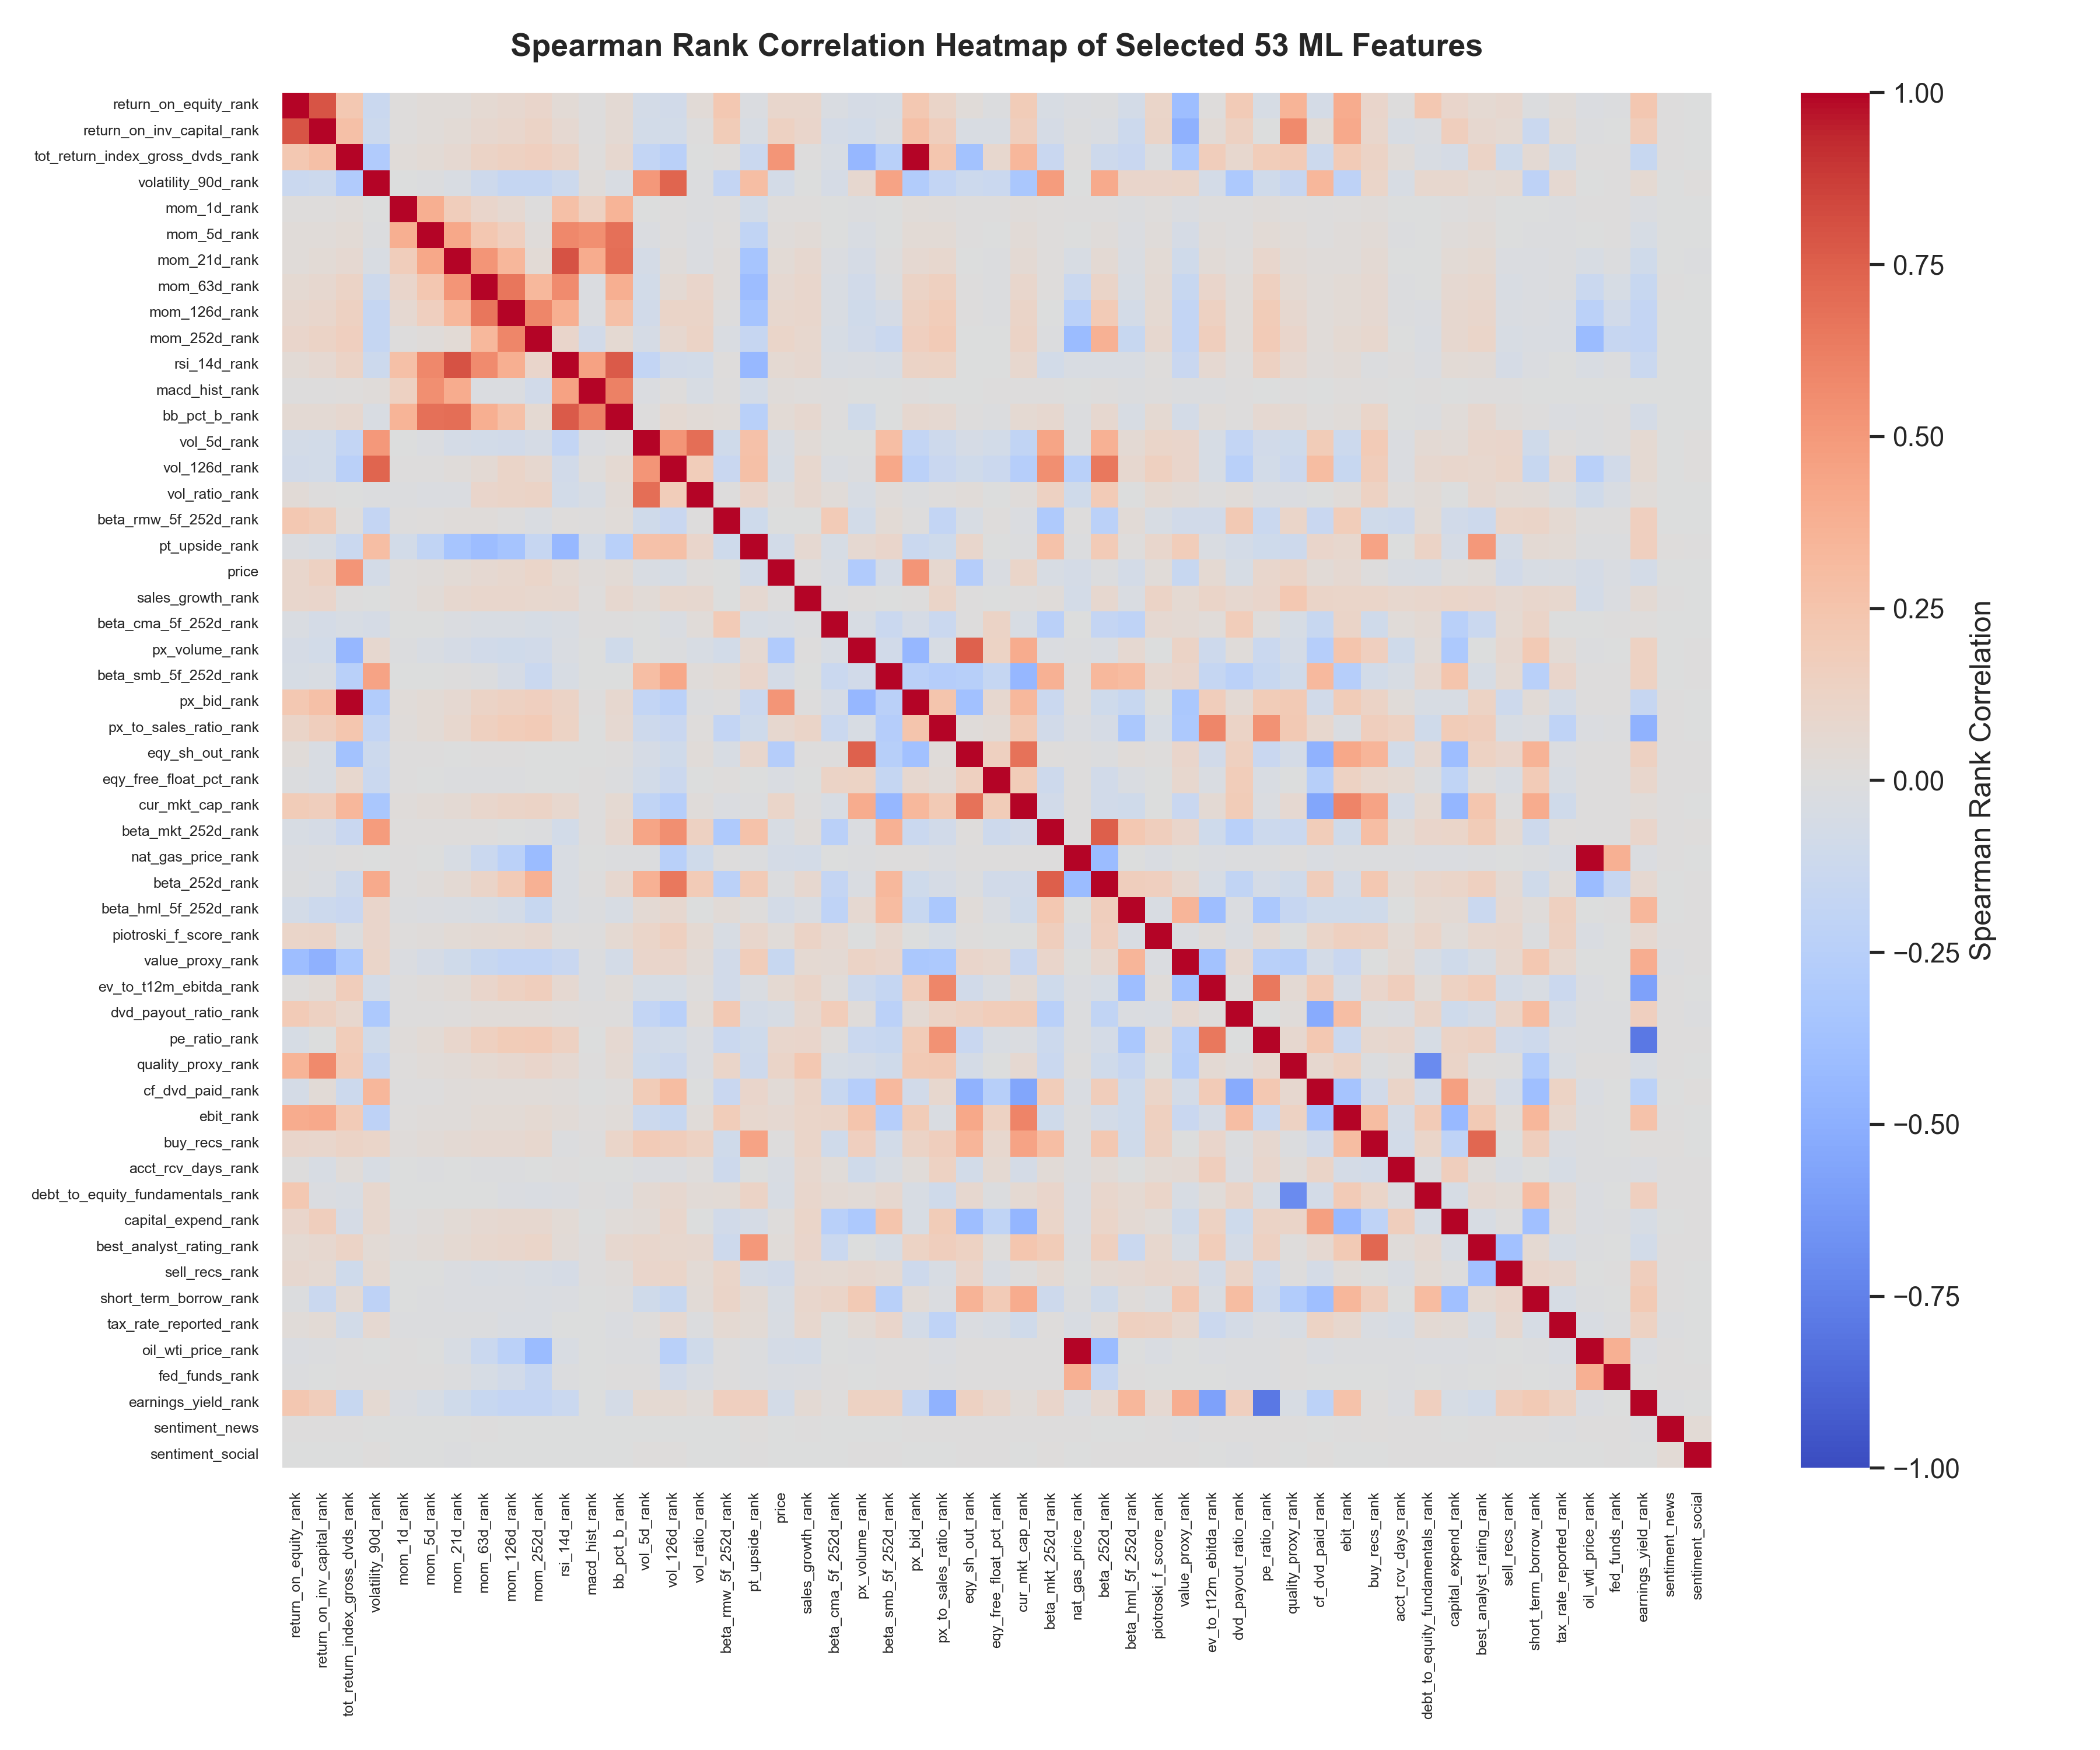
\includegraphics[width=0.80\textwidth]{./figures/selected_features_correlation.png}
\vspace{-0.2cm}
\caption{Spearman Rank Correlation Heatmap of Selected 53 ML Features}
\label{fig:ch3_corr_heatmap}
\end{figure}

\begin{figure}[htbp]
\centering
\vspace{-0.2cm}
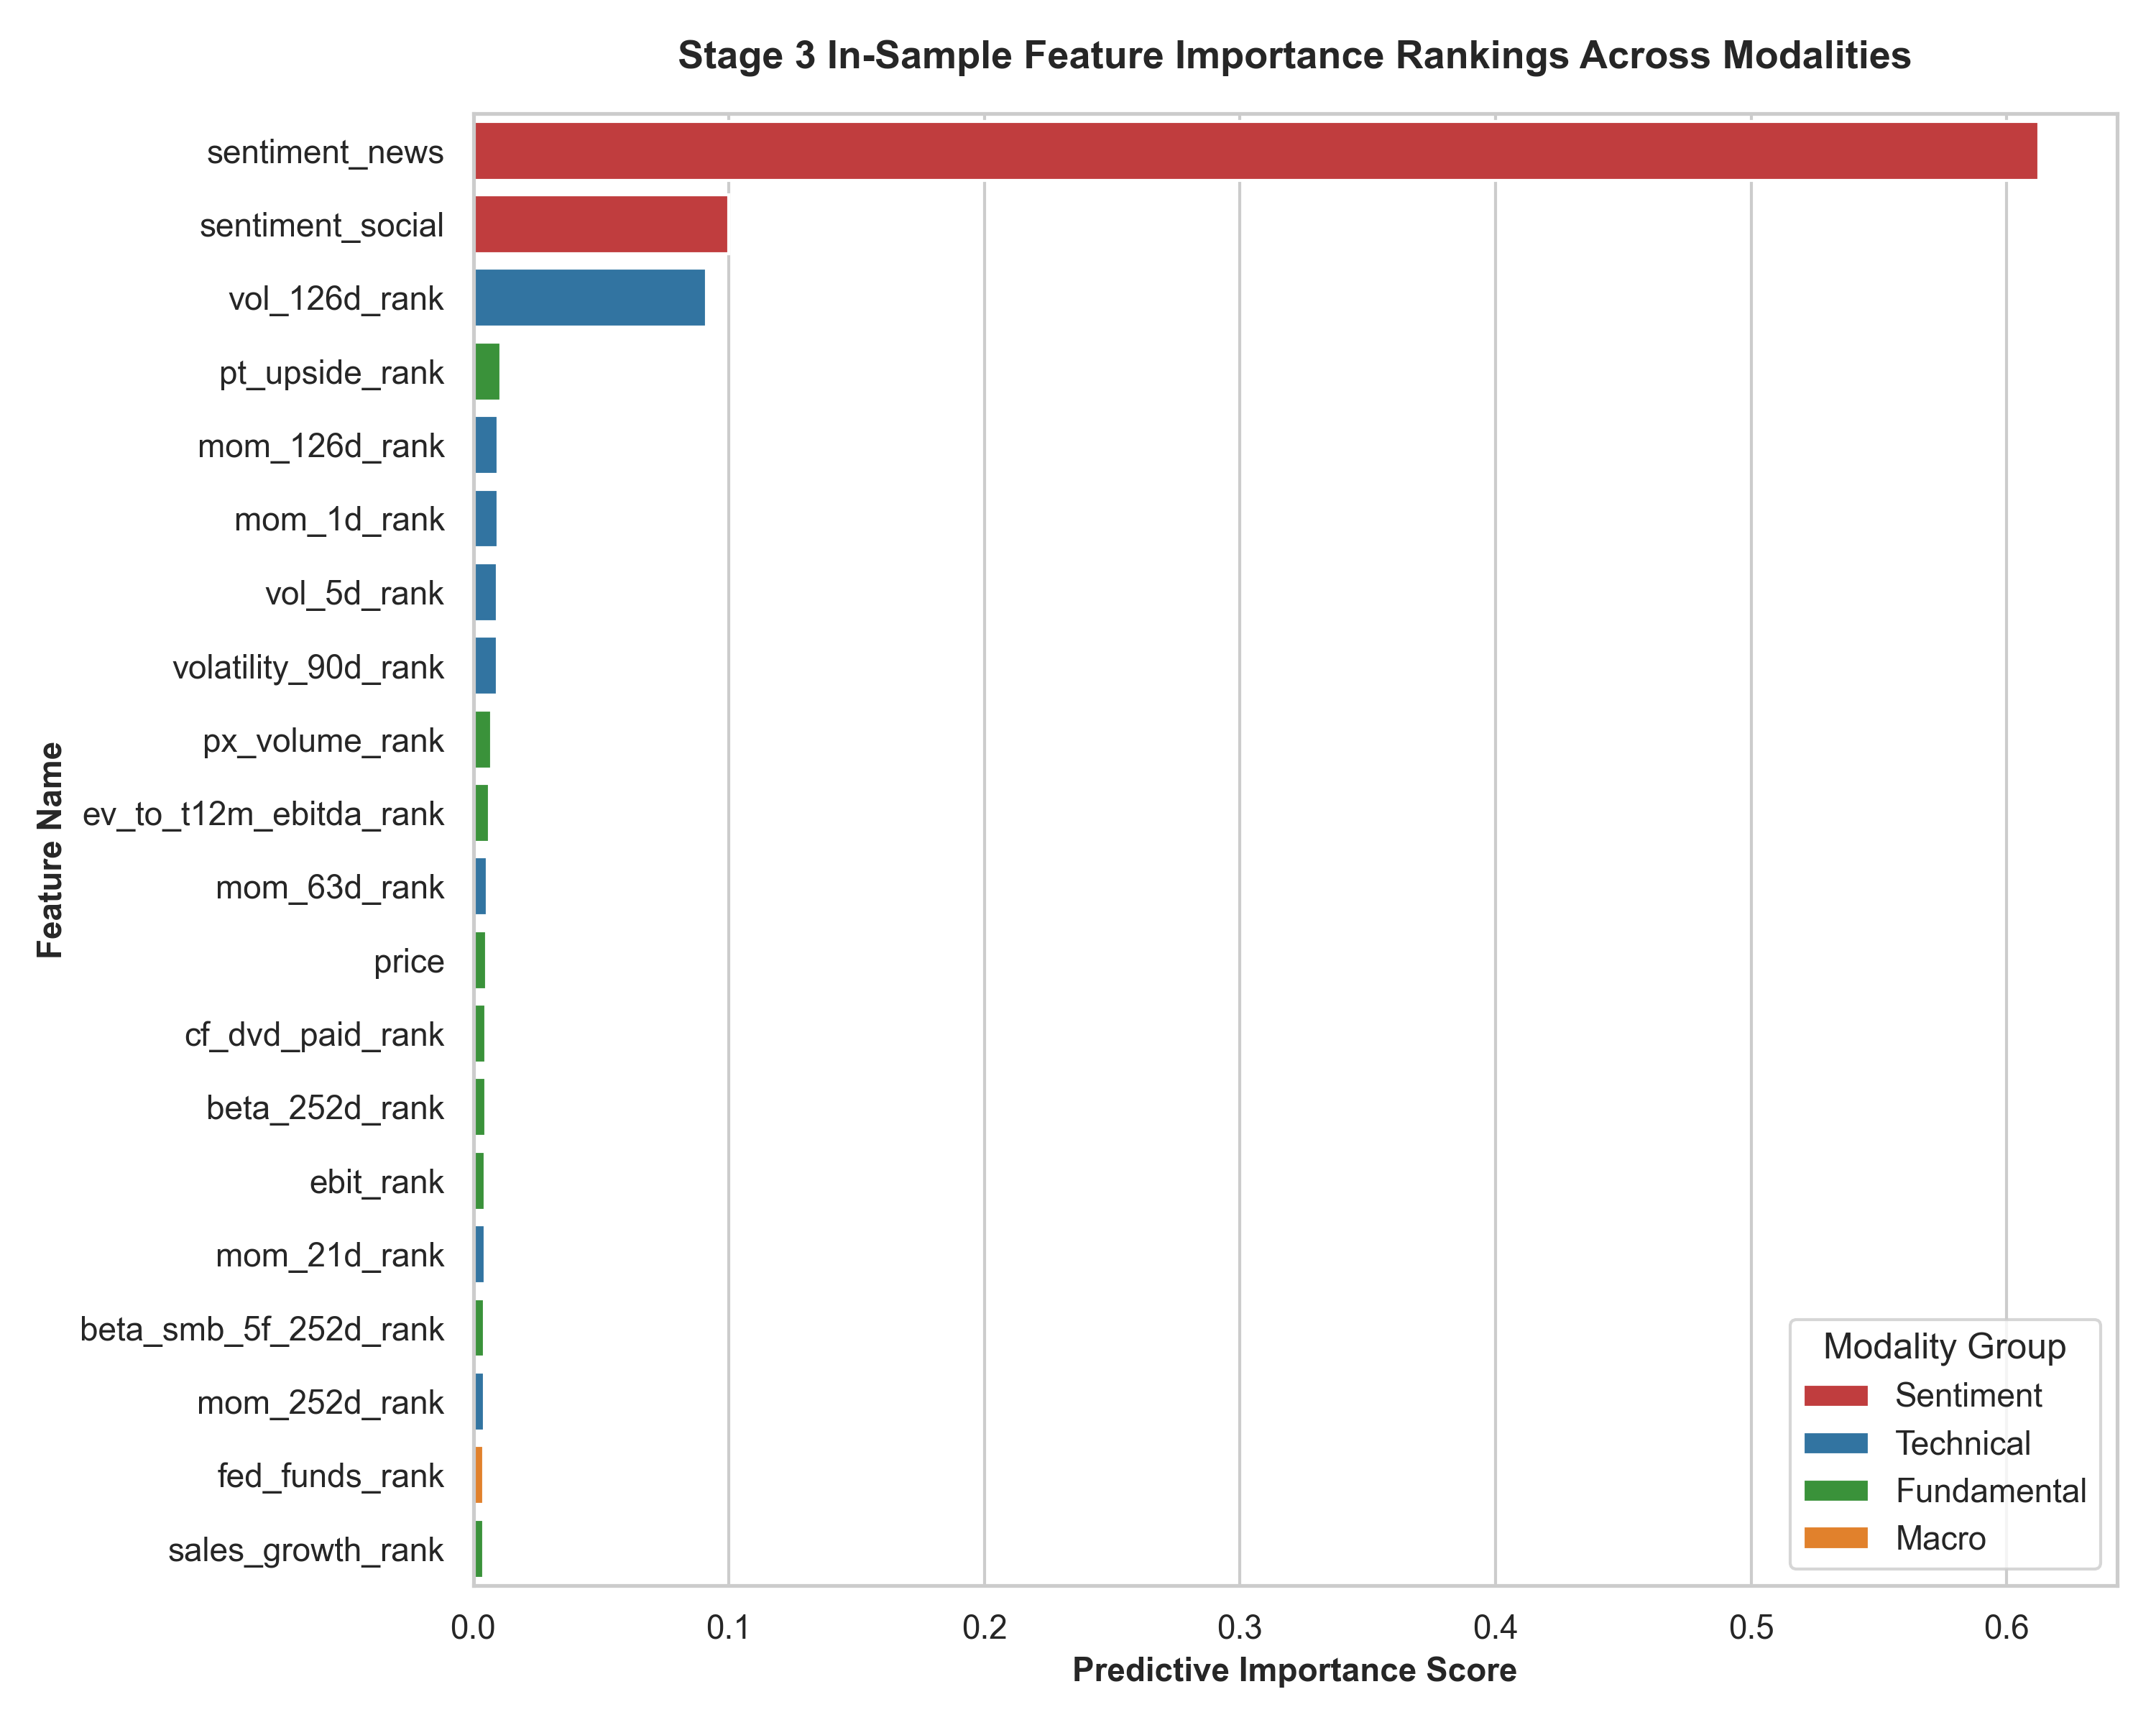
\includegraphics[width=0.80\textwidth]{./figures/selected_feature_importances.png}
\vspace{-0.2cm}
\caption{Stage 3 In-Sample Permutation Feature Importance Rankings across Modalities}
\label{fig:ch3_rf_importance}
\end{figure}

Figure \ref{fig:ch3_rf_importance} reports the in-sample permutation feature importances calculated strictly on pre-2020 training data to prevent out-of-sample lookahead leakage. A classic methodological issue in tree-based feature selection is that raw Gini impurity measures over-attribute importance to continuous, un-normalized variables \citep{strobl2007bias}. Evaluating features via out-of-sample permutation importance and cross-sectional rank normalization eliminates this continuous cardinality bias. Technical momentum indicators ($\text{vol}_{126d}$, $\text{mom}_{21d}$, $\text{rsi}_{14d}$) and fundamental metrics ($\text{pe}_{\text{ratio}}$, $\text{roi}$, $\text{quality}$) emerge as the dominant predictive drivers, while sentiment indicators provide moderate secondary refinement, aligning fully with downstream SHAP values (Figure \ref{fig:ch4_shap_summary}) and modality ablation evidence (Table \ref{tab:ch4_ablation_study}).

\section{Baseline Econometric \& Machine Learning Formulations}
\label{sec:ch3_baselines}

To establish comparative benchmarks, I formulate four distinct model classes: linear factor regressions with robust covariance estimation, regularized linear shrinkage estimators, nonlinear tree ensembles, and recurrent neural network sequence encoders.

\subsection{Fama-MacBeth 2-Pass Linear Regression \& Newey-West HAC Estimation}
\label{subsec:ch3_fama_macbeth}

The benchmark linear asset pricing model follows the two-pass cross-sectional regression procedure of \citet{fama1973risk}, incorporating 1-day lagged factor loadings to prevent lookahead bias and heteroskedasticity and autocorrelation consistent (HAC) covariance matrices \citep{newey1987simple}.

\subsubsection{Pass 1: Rolling Time-Series Factor Loading Estimation}
For each individual stock $i \in \{1, \dots, N_t\}$ on trading day $t$, factor loadings (betas) are estimated over a rolling historical lookback window of $W = 252$ trading days (one calendar year). Let $\mathbf{R}_{i,t} = [R_{i, t-W+1}, R_{i, t-W+2}, \dots, R_{i,t}]^T \in \mathbb{R}^{W \times 1}$ denote the vector of historical daily excess returns for asset $i$, and let $\mathbf{F}_t \in \mathbb{R}^{W \times (K+1)}$ represent the matrix of $K$ benchmark factor returns plus a column of ones for the intercept:
\begin{equation}
\resizebox{0.88\textwidth}{!}{$
\mathbf{F}_t = \begin{bmatrix}
1 & F_{1,\, t-W+1} & F_{2,\, t-W+1} & \cdots & F_{K,\, t-W+1} \\
1 & F_{1,\, t-W+2} & F_{2,\, t-W+2} & \cdots & F_{K,\, t-W+2} \\
\vdots & \vdots & \vdots & \ddots & \vdots \\
1 & F_{1,\, t} & F_{2,\, t} & \cdots & F_{K,\, t}
\end{bmatrix}
$}
\end{equation}

The first-pass time series Ordinary Least Squares (OLS) regression for stock $i$ is formulated as:
\begin{equation}
\mathbf{R}_{i,t} = \mathbf{F}_t \boldsymbol{\beta}_{i,t} + \boldsymbol{\epsilon}_{i,t}
\label{eq:ch3_pass1_ols}
\end{equation}
where $\boldsymbol{\beta}_{i,t} = [\alpha_{i,t}, \beta_{i,1,t}, \beta_{i,2,t}, \dots, \beta_{i,K,t}]^T \in \mathbb{R}^{(K+1) \times 1}$. The OLS point estimator is obtained by minimizing the sum of squared residuals:
\begin{equation}
\hat{\boldsymbol{\beta}}_{i,t} = \arg\min_{\boldsymbol{\beta}} (\mathbf{R}_{i,t} - \mathbf{F}_t \boldsymbol{\beta})^T (\mathbf{R}_{i,t} - \mathbf{F}_t \boldsymbol{\beta}) = \left( \mathbf{F}_t^T \mathbf{F}_t \right)^{-1} \mathbf{F}_t^T \mathbf{R}_{i,t}
\label{eq:ch3_beta_hat}
\end{equation}
To enforce zero-lookahead protection, factor loadings $\hat{\boldsymbol{\beta}}_{i,t}$ estimated using data up to day $t$ are indexed to predict returns at day $t+1$.

\subsubsection{Pass 2: Daily Cross-Sectional Factor Risk Premia Estimation}
On each trading day $t+1$, a cross-sectional OLS regression is estimated across all active constituent assets $N_{t+1}$ using the 1-day lagged factor loadings $\hat{\mathbf{B}}_t = [\mathbf{1}, \hat{\boldsymbol{\beta}}_{1,t}, \hat{\boldsymbol{\beta}}_{2,t}, \dots, \hat{\boldsymbol{\beta}}_{N_{t+1},t}]^T \in \mathbb{R}^{N_{t+1} \times (K+1)}$:
\begin{equation}
\mathbf{R}_{t+1} = \hat{\mathbf{B}}_t \boldsymbol{\gamma}_{t+1} + \boldsymbol{\eta}_{t+1}
\label{eq:ch3_pass2_ols}
\end{equation}
where $\mathbf{R}_{t+1} = [R_{1,t+1}, R_{2,t+1}, \dots, R_{N_{t+1},t+1}]^T \in \mathbb{R}^{N_{t+1} \times 1}$ is the cross-section of realized forward returns, $\boldsymbol{\gamma}_{t+1} = [\gamma_{0,t+1}, \gamma_{1,t+1}, \dots, \gamma_{K,t+1}]^T \in \mathbb{R}^{(K+1) \times 1}$ represents the vector of daily factor risk premia (and cross-sectional intercept $\gamma_{0,t+1}$), and $\boldsymbol{\eta}_{t+1}$ is the vector of cross-sectional pricing errors.

The closed-form daily cross-sectional risk premium estimator is given by:
\begin{equation}
\hat{\boldsymbol{\gamma}}_{t+1} = \left( \hat{\mathbf{B}}_t^T \hat{\mathbf{B}}_t \right)^{-1} \hat{\mathbf{B}}_t^T \mathbf{R}_{t+1}
\label{eq:ch3_gamma_hat}
\end{equation}

\subsubsection{Time-Series Aggregation \& Step-by-Step Newey-West HAC Proof}
Over an evaluation period of $T$ trading days, the overall factor risk premium vector is estimated as the sample mean across daily cross-sectional estimates:
\begin{equation}
\bar{\boldsymbol{\gamma}} = \frac{1}{T} \sum_{t=1}^T \hat{\boldsymbol{\gamma}}_t
\end{equation}

Because daily factor risk premia estimates $\hat{\boldsymbol{\gamma}}_t$ suffer from serial correlation (autocorrelation) due to overlapping return measurement horizons and conditional heteroskedasticity in asset volatility, standard i.i.d. variance estimators underestimate true standard errors, inflating test statistics.

To derive a consistent estimator for the asymptotic covariance matrix of $\bar{\boldsymbol{\gamma}}$, let $\mathbf{u}_t = \hat{\boldsymbol{\gamma}}_t - \bar{\boldsymbol{\gamma}} \in \mathbb{R}^{(K+1) \times 1}$ denote the vector of mean-zero risk premium innovations. The variance of the sample average factor risk premium is:
\begin{equation}
\operatorname{Var}(\bar{\boldsymbol{\gamma}}) = \operatorname{Var}\left( \frac{1}{T} \sum_{t=1}^T \hat{\boldsymbol{\gamma}}_t \right) = \frac{1}{T^2} \sum_{t=1}^T \sum_{s=1}^T \mathbb{E}\left[ \mathbf{u}_t \mathbf{u}_s^T \right]
\label{eq:ch3_var_gamma_sum}
\end{equation}
Defining the sample autocovariance matrix at lag $j$ as:
\begin{equation}
\hat{\mathbf{\Gamma}}_j = \frac{1}{T} \sum_{t=j+1}^T \mathbf{u}_t \mathbf{u}_{t-j}^T, \quad \text{for } j \ge 0
\label{eq:ch3_autocovariance}
\end{equation}
Equation (\ref{eq:ch3_var_gamma_sum}) can be expanded into the sum of zero-lag covariance and off-diagonal cross-lag covariances:
\begin{equation}
\operatorname{Var}(\bar{\boldsymbol{\gamma}}) = \frac{1}{T} \left[ \hat{\mathbf{\Gamma}}_0 + \sum_{j=1}^{T-1} \left( \hat{\mathbf{\Gamma}}_j + \hat{\mathbf{\Gamma}}_j^T \right) \right]
\end{equation}

Unweighted truncation of lag covariances at finite lag $L < T$ can lead to non-positive semi-definite covariance matrices in finite samples. The \citet{newey1987simple} HAC covariance matrix estimator guarantees positive semi-definiteness by weighting lag autocovariances with the triangular Bartlett kernel $w(j,L)$:
\begin{equation}
\widehat{\mathbf{\Omega}}_{\text{HAC}} = \hat{\mathbf{\Gamma}}_0 + \sum_{j=1}^L w(j, L) \left( \hat{\mathbf{\Gamma}}_j + \hat{\mathbf{\Gamma}}_j^T \right)
\label{eq:ch3_newey_west_omega}
\end{equation}
where the Bartlett kernel weights are defined as:
\begin{equation}
w(j, L) = 1 - \frac{j}{L+1}, \quad j = 1, 2, \dots, L
\label{eq:ch3_bartlett_kernel}
\end{equation}
and the lag truncation bandwidth $L$ is set according to the bandwidth selection rule $L = \lfloor 4 (T / 100)^{2/9} \rfloor$.

\begin{proof}[Proof of Guaranteed Positive Semi-Definiteness]
To prove that $\widehat{\mathbf{\Omega}}_{\text{HAC}} \succeq 0$, express the Bartlett kernel as the spectral window resulting from the convolution of a rectangular sequence with itself. Define $\mathbf{u}_t = \mathbf{0}$ for $t \notin \{1, \dots, T\}$. Consider the smoothed sequence $\mathbf{s}_t = \frac{1}{\sqrt{L+1}} \sum_{m=0}^L \mathbf{u}_{t+m}$. The sample covariance of $\mathbf{s}_t$ is positive semi-definite:
\begin{align}
\mathbf{M} &= \frac{1}{T} \sum_{t=-\infty}^{\infty} \mathbf{s}_t \mathbf{s}_t^T = \frac{1}{T(L+1)} \sum_{t=-\infty}^{\infty} \left( \sum_{m=0}^L \mathbf{u}_{t+m} \right) \left( \sum_{n=0}^L \mathbf{u}_{t+n}^T \right) \ge 0
\end{align}
Expanding the double summation yields:
\begin{align}
\mathbf{M} &= \frac{1}{T(L+1)} \sum_{m=0}^L \sum_{n=0}^L \sum_{t=-\infty}^{\infty} \mathbf{u}_{t+m} \mathbf{u}_{t+n}^T = \frac{1}{T(L+1)} \sum_{m=0}^L \sum_{n=0}^L T \hat{\mathbf{\Gamma}}_{m-n} \\
&= \frac{1}{L+1} \sum_{k=-L}^L (L + 1 - |k|) \hat{\mathbf{\Gamma}}_k = \hat{\mathbf{\Gamma}}_0 + \sum_{j=1}^L \left( 1 - \frac{j}{L+1} \right) \left( \hat{\mathbf{\Gamma}}_j + \hat{\mathbf{\Gamma}}_j^T \right) = \widehat{\mathbf{\Omega}}_{\text{HAC}}
\end{align}
Since $\mathbf{M}$ is constructed as a sum of outer products $\mathbf{s}_t \mathbf{s}_t^T$, for any vector $\mathbf{a} \in \mathbb{R}^{K+1}$, $\mathbf{a}^T \widehat{\mathbf{\Omega}}_{\text{HAC}} \mathbf{a} = \frac{1}{T} \sum_t (\mathbf{a}^T \mathbf{s}_t)^2 \ge 0$. Thus, $\widehat{\mathbf{\Omega}}_{\text{HAC}}$ is positive semi-definite.
\end{proof}

The Newey-West adjusted standard error for the $k$-th factor risk premium estimate $\bar{\gamma}_k$ is:
\begin{equation}
\text{SE}_{\text{NW}}(\bar{\gamma}_k) = \sqrt{ \frac{1}{T} \left[ \widehat{\mathbf{\Omega}}_{\text{HAC}} \right]_{kk} }
\end{equation}
and the test statistic for factor significance testing is evaluated as $t(\bar{\gamma}_k) = \frac{\bar{\gamma}_k}{\text{SE}_{\text{NW}}(\bar{\gamma}_k)}$.

\subsection{Regularized Linear Models: ElasticNet, LASSO, \& Ridge}
\label{subsec:ch3_elasticnet_lasso_ridge}

High dimensional cross-sectional asset pricing settings with $P$ characteristic features suffer from multicollinearity and sample overfitting under standard OLS. Regularized linear models introduce penalty structures to constrain coefficient magnitudes and perform feature selection \citep{kozak2020shrinking}.

\subsubsection{ElasticNet Objective Function}
Let $\mathbf{y} \in \mathbb{R}^N$ denote the vector of standardized forward returns across all asset-day observations, and let $\mathbf{X} \in \mathbb{R}^{N \times P}$ denote the matrix of standardized stock characteristics. The ElasticNet estimator \citep{zou2005regularization} solves the convex optimization problem:
\begin{equation}
\min_{\boldsymbol{\beta} \in \mathbb{R}^P} \mathcal{L}_{\text{EN}}(\boldsymbol{\beta}) = \frac{1}{2N} \|\mathbf{y} - \mathbf{X}\boldsymbol{\beta}\|_2^2 + \lambda \left[ \alpha \|\boldsymbol{\beta}\|_1 + \frac{1-\alpha}{2} \|\boldsymbol{\beta}\|_2^2 \right]
\label{eq:ch3_elasticnet_full}
\end{equation}
where $\lambda > 0$ controls the penalty intensity, $\alpha \in [0, 1]$ governs the ratio between the $L_1$ norm $\|\boldsymbol{\beta}\|_1 = \sum_{j=1}^P |\beta_j|$ and the squared $L_2$ norm $\|\boldsymbol{\beta}\|_2^2 = \sum_{j=1}^P \beta_j^2$. Setting $\alpha = 1.0$ yields the LASSO estimator \citep{tibshirani1996regression}, while $\alpha = 0.0$ yields Ridge regression \citep{hoerl1970ridge}.

\subsubsection{Subgradient Calculus \& Characterization of LASSO ($L_1$) Sparsity}
Because the $L_1$ norm is non-differentiable at $\beta_j = 0$, optimization requires subgradient calculus. The subdifferential $\partial |\beta_j|$ of the absolute value function is defined as:
\begin{equation}
\partial |\beta_j| = \begin{cases} 
\{ +1 \} & \text{if } \beta_j > 0 \\
\{ -1 \} & \text{if } \beta_j < 0 \\
[-1, 1] & \text{if } \beta_j = 0 
\end{cases}
\label{eq:ch3_subgradient_l1}
\end{equation}

To derive the coordinate descent update rule for feature $j$, assume that the columns of $\mathbf{X}$ are standardized such that $\mathbf{x}_j^T \mathbf{x}_j = N$. Isolate feature $j$ by defining the partial residual vector $\mathbf{r}^{(j)} = \mathbf{y} - \sum_{k \neq j} \mathbf{x}_k \beta_k$. The unregularized OLS update for $\beta_j$ given fixed $\boldsymbol{\beta}_{-j}$ is $\hat{\beta}_j^{\text{OLS}} = \frac{1}{N} \mathbf{x}_j^T \mathbf{r}^{(j)}$.

The first order optimality condition for the ElasticNet objective requires $0 \in \partial_{\beta_j} \mathcal{L}_{\text{EN}}(\boldsymbol{\beta})$:
\begin{equation}
-\frac{1}{N} \mathbf{x}_j^T (\mathbf{y} - \mathbf{X}\boldsymbol{\beta}) + \lambda(1-\alpha)\beta_j + \lambda \alpha v_j = 0, \quad \text{where } v_j \in \partial |\beta_j|
\end{equation}
Substituting $\mathbf{y} - \mathbf{X}\boldsymbol{\beta} = \mathbf{r}^{(j)} - \mathbf{x}_j \beta_j$ and using $\frac{1}{N}\mathbf{x}_j^T \mathbf{x}_j = 1$:
\begin{equation}
-\hat{\beta}_j^{\text{OLS}} + \beta_j + \lambda(1-\alpha)\beta_j + \lambda \alpha v_j = 0 \implies \beta_j [ 1 + \lambda(1-\alpha) ] + \lambda \alpha v_j = \hat{\beta}_j^{\text{OLS}}
\label{eq:ch3_opt_condition}
\end{equation}

Solving Equation (\ref{eq:ch3_opt_condition}) under three case conditions for $\hat{\beta}_j^{\text{OLS}}$:
\begin{enumerate}
    \item \textbf{Case 1: $\beta_j > 0$}. Here $v_j = +1$. Equation (\ref{eq:ch3_opt_condition}) gives $\beta_j [1 + \lambda(1-\alpha)] = \hat{\beta}_j^{\text{OLS}} - \lambda \alpha$, requiring $\hat{\beta}_j^{\text{OLS}} > \lambda \alpha$. Thus:
    $$\beta_j^* = \frac{\hat{\beta}_j^{\text{OLS}} - \lambda \alpha}{1 + \lambda(1-\alpha)}$$
    \item \textbf{Case 2: $\beta_j < 0$}. Here $v_j = -1$. Equation (\ref{eq:ch3_opt_condition}) gives $\beta_j [1 + \lambda(1-\alpha)] = \hat{\beta}_j^{\text{OLS}} + \lambda \alpha$, requiring $\hat{\beta}_j^{\text{OLS}} < -\lambda \alpha$. Thus:
    $$\beta_j^* = \frac{\hat{\beta}_j^{\text{OLS}} + \lambda \alpha}{1 + \lambda(1-\alpha)}$$
    \item \textbf{Case 3: $\beta_j = 0$}. Here $v_j \in [-1, 1]$. Equation (\ref{eq:ch3_opt_condition}) requires $|\hat{\beta}_j^{\text{OLS}}| \le \lambda \alpha$. Thus, $\beta_j^* = 0$.
\end{enumerate}

Combining these cases yields the closed-form Soft-Thresholding Operator $\mathcal{S}_{\kappa}(z) = \operatorname{sign}(z) \max(0, |z| - \kappa)$:
\begin{equation}
\hat{\beta}_j^{\text{EN}} = \frac{\mathcal{S}_{\lambda \alpha}\left( \hat{\beta}_j^{\text{OLS}} \right)}{1 + \lambda (1-\alpha)}
\label{eq:ch3_soft_thresholding_en}
\end{equation}
Setting $\alpha = 1.0$ yields the standard LASSO soft-thresholded estimator $\hat{\beta}_j^{\text{LASSO}} = \mathcal{S}_{\lambda}\left( \hat{\beta}_j^{\text{OLS}} \right)$, which sets coefficients to zero whenever $|\hat{\beta}_j^{\text{OLS}}| \le \lambda$, performing feature selection.

\subsubsection{Ridge ($L_2$) Shrinkage Bounds \& SVD Derivation}
For Ridge regression ($\alpha = 0$), the objective function is smooth and differentiable. Differentiating $\mathcal{L}_{\text{Ridge}}(\boldsymbol{\beta})$ with respect to $\boldsymbol{\beta}$ yields the closed-form Ridge estimator:
\begin{equation}
\hat{\boldsymbol{\beta}}_{\text{Ridge}} = \left( \mathbf{X}^T \mathbf{X} + N \lambda \mathbf{I}_P \right)^{-1} \mathbf{X}^T \mathbf{y}
\label{eq:ch3_ridge_closed_form}
\end{equation}

To derive $L_2$ shrinkage bounds, consider the Singular Value Decomposition (SVD) of the centered design matrix $\mathbf{X} = \mathbf{U} \mathbf{\Sigma} \mathbf{V}^T$, where $\mathbf{U} \in \mathbb{R}^{N \times P}$ and $\mathbf{V} \in \mathbb{R}^{P \times P}$ are orthonormal matrices ($\mathbf{U}^T \mathbf{U} = \mathbf{I}_P$, $\mathbf{V}^T \mathbf{V} = \mathbf{I}_P$), and $\mathbf{\Sigma} = \operatorname{diag}(\sigma_1, \sigma_2, \dots, \sigma_P)$ contains the singular values $\sigma_1 \ge \sigma_2 \ge \dots \ge \sigma_P > 0$.

Substituting the SVD into the standard OLS estimator $\hat{\boldsymbol{\beta}}_{\text{OLS}} = (\mathbf{X}^T \mathbf{X})^{-1} \mathbf{X}^T \mathbf{y}$:
\begin{equation}
\hat{\boldsymbol{\beta}}_{\text{OLS}} = \left( \mathbf{V} \mathbf{\Sigma}^2 \mathbf{V}^T \right)^{-1} \mathbf{V} \mathbf{\Sigma} \mathbf{U}^T \mathbf{y} = \mathbf{V} \mathbf{\Sigma}^{-1} \mathbf{U}^T \mathbf{y}
\end{equation}

Substituting the SVD into the Ridge estimator Equation (\ref{eq:ch3_ridge_closed_form}):
\begin{align}
\hat{\boldsymbol{\beta}}_{\text{Ridge}} &= \left( \mathbf{V} \mathbf{\Sigma}^2 \mathbf{V}^T + N \lambda \mathbf{V} \mathbf{I}_P \mathbf{V}^T \right)^{-1} \mathbf{V} \mathbf{\Sigma} \mathbf{U}^T \mathbf{y} \\
&= \left( \mathbf{V} [ \mathbf{\Sigma}^2 + N \lambda \mathbf{I}_P ] \mathbf{V}^T \right)^{-1} \mathbf{V} \mathbf{\Sigma} \mathbf{U}^T \mathbf{y} \\
&= \mathbf{V} \left( \mathbf{\Sigma}^2 + N \lambda \mathbf{I}_P \right)^{-1} \mathbf{\Sigma} \mathbf{U}^T \mathbf{y}
\label{eq:ch3_ridge_svd}
\end{align}

Expressing $\hat{\boldsymbol{\beta}}_{\text{Ridge}}$ directly as a transformation of the unregularized OLS estimator $\hat{\boldsymbol{\beta}}_{\text{OLS}}$:
\begin{align}
\hat{\boldsymbol{\beta}}_{\text{Ridge}} &= \mathbf{V} \left( \mathbf{\Sigma}^2 + N \lambda \mathbf{I}_P \right)^{-1} \mathbf{\Sigma}^2 \mathbf{\Sigma}^{-1} \mathbf{U}^T \mathbf{y} \\
&= \mathbf{V} \operatorname{diag}\left( \frac{\sigma_j^2}{\sigma_j^2 + N \lambda} \right) \mathbf{V}^T \hat{\boldsymbol{\beta}}_{\text{OLS}}
\label{eq:ch3_ridge_shrinkage_matrix}
\end{align}

Because $N \lambda > 0$ and $\sigma_j^2 > 0$, the shrinkage factor satisfies:
\begin{equation}
0 < \frac{\sigma_j^2}{\sigma_j^2 + N \lambda} < 1, \quad \forall j \in \{1, \dots, P\}
\end{equation}
This shows that Ridge regression shrinks the OLS parameter vector along the principal component directions of $\mathbf{X}$, with greater shrinkage applied to components with smaller singular values $\sigma_j^2$. Consequently, $\|\hat{\boldsymbol{\beta}}_{\text{Ridge}}\|_2 < \|\hat{\boldsymbol{\beta}}_{\text{OLS}}\|_2$ for all $\lambda > 0$, bounding parameter variance and stabilizing prediction under collinearity.

\subsection{Non-Linear Tree Ensembles: Random Forest \& XGBoost}
\label{subsec:ch3_tree_ensembles}

Decision tree ensembles map high dimensional characteristic spaces into predicted returns by partitioning features into hyper-rectangular regions \citep{gu2020empirical}.

\subsubsection{Random Forest Bagging Variance Reduction Proof}
The Random Forest regressor \citep{breiman2001random} constructs an ensemble of $M$ decorrelated decision trees $\{T_1(\mathbf{x}), T_2(\mathbf{x}), \dots, T_M(\mathbf{x})\}$, each trained on a bootstrap sample of size $N$ with randomized feature subspace selection ($m_{\text{try}}$). While the classic \citet{breiman2001random} rule of thumb sets $m_{\text{try}} = \lfloor \sqrt{P} \rfloor = \lfloor \sqrt{53} \rfloor = 7$ (a feature subsample ratio of $7/53 \approx 0.13$), cross-validation tuning across expanding folds yields an optimal ratio of $m_{\text{try}}/P = 0.40$ ($m_{\text{try}} = 21$ features per node split), which prevents under-fitting when features are correlated within modalities. The ensemble prediction is the average:
\begin{equation}
\hat{f}_{\text{RF}}(\mathbf{x}) = \frac{1}{M} \sum_{m=1}^M T_m(\mathbf{x})
\label{eq:ch3_rf_prediction}
\end{equation}

Assume each individual tree $T_m(\mathbf{x})$ is identically distributed with variance $\operatorname{Var}(T_m(\mathbf{x})) = \sigma^2$, and that any pair of distinct trees $(T_m, T_l)$ for $m \neq l$ has pairwise correlation $\text{Corr}(T_m(\mathbf{x}), T_l(\mathbf{x})) = \rho$.

\begin{proof}[Proof of Variance Reduction Dynamics]
Compute the variance of the ensemble estimator $\hat{f}_{\text{RF}}(\mathbf{x})$:
\begin{align}
\operatorname{Var}\left( \hat{f}_{\text{RF}}(\mathbf{x}) \right) &= \operatorname{Var}\left( \frac{1}{M} \sum_{m=1}^M T_m(\mathbf{x}) \right) \\
&= \frac{1}{M^2} \left[ \sum_{m=1}^M \operatorname{Var}(T_m(\mathbf{x})) + \sum_{m=1}^M \sum_{l \neq m}^M \operatorname{Cov}(T_m(\mathbf{x}), T_l(\mathbf{x})) \right]
\label{eq:ch3_var_rf_expansion}
\end{align}
Substitute $\operatorname{Var}(T_m(\mathbf{x})) = \sigma^2$ and $\operatorname{Cov}(T_m(\mathbf{x}), T_l(\mathbf{x})) = \rho \sigma^2$:
\begin{align}
\operatorname{Var}\left( \hat{f}_{\text{RF}}(\mathbf{x}) \right) &= \frac{1}{M^2} \left[ M \sigma^2 + M(M-1) \rho \sigma^2 \right] \\
&= \frac{\sigma^2}{M} + \frac{M-1}{M} \rho \sigma^2 = \rho \sigma^2 + \frac{1 - \rho}{M} \sigma^2
\label{eq:ch3_var_rf_final}
\end{align}
\end{proof}

Taking the limit as the number of trees $M \to \infty$:
\begin{equation}
\lim_{M \to \infty} \operatorname{Var}\left( \hat{f}_{\text{RF}}(\mathbf{x}) \right) = \rho \sigma^2
\end{equation}
Equation (\ref{eq:ch3_var_rf_final}) demonstrates the variance-reduction mechanism of Random Forest:
\begin{enumerate}
    \item \textbf{Bagging} (bootstrap aggregation) reduces the term $\frac{1-\rho}{M} \sigma^2$ toward zero as the ensemble size $M$ increases.
    \item \textbf{Random Feature Subspace Selection} reduces inter-tree correlation $\rho$, lowering the variance floor $\rho \sigma^2$.
\end{enumerate}

\subsubsection{XGBoost Second-Order Taylor Expansion Loss Optimization}
Extreme Gradient Boosting (XGBoost) \citep{chen2016xgboost} builds an additive model of $M$ decision trees sequentially: $\hat{y}_i^{(m)} = \hat{y}_i^{(m-1)} + f_m(\mathbf{x}_i)$. At step $m$, the regularized objective function to minimize is:
\begin{equation}
\mathcal{L}^{(m)} = \sum_{i=1}^N l\left( y_i, \hat{y}_i^{(m-1)} + f_m(\mathbf{x}_i) \right) + \Omega(f_m)
\label{eq:ch3_xgb_obj}
\end{equation}
where $l(\cdot, \cdot)$ is a differentiable convex loss function, and the tree complexity regularization term $\Omega(f_m)$ is defined for a tree with $T$ leaf nodes and leaf weight vector $\mathbf{w} = [w_1, \dots, w_T]^T \in \mathbb{R}^T$ as:
\begin{equation}
\Omega(f_m) = \gamma T + \frac{1}{2} \lambda \|\mathbf{w}\|_2^2 = \gamma T + \frac{1}{2} \lambda \sum_{j=1}^T w_j^2
\label{eq:ch3_xgb_reg}
\end{equation}

Applying a second order Taylor expansion to the loss function around the previous iteration forecast $\hat{y}_i^{(m-1)}$:
\begin{equation}
l\left( y_i, \hat{y}_i^{(m-1)} + f_m(\mathbf{x}_i) \right) \approx l\left( y_i, \hat{y}_i^{(m-1)} \right) + g_i f_m(\mathbf{x}_i) + \frac{1}{2} h_i f_m(\mathbf{x}_i)^2
\label{eq:ch3_taylor_loss}
\end{equation}
where the first order gradient $g_i$ and second order Hessian $h_i$ are defined as:
\begin{equation}
g_i = \frac{\partial l\left( y_i, \hat{y}_i^{(m-1)} \right)}{\partial \hat{y}_i^{(m-1)}}, \quad h_i = \frac{\partial^2 l\left( y_i, \hat{y}_i^{(m-1)} \right)}{\partial \left(\hat{y}_i^{(m-1)}\right)^2}
\label{eq:ch3_grad_hessian}
\end{equation}

Removing constant terms $l(y_i, \hat{y}_i^{(m-1)})$ independent of tree structure $f_m$, the simplified objective at step $m$ becomes:
\begin{equation}
\tilde{\mathcal{L}}^{(m)} = \sum_{i=1}^N \left[ g_i f_m(\mathbf{x}_i) + \frac{1}{2} h_i f_m(\mathbf{x}_i)^2 \right] + \gamma T + \frac{1}{2} \lambda \sum_{j=1}^T w_j^2
\label{eq:ch3_xgb_simplified_obj}
\end{equation}

Let $I_j = \{i \mid q(\mathbf{x}_i) = j\}$ represent the instance set mapped to leaf node $j$ by structure mapping function $q: \mathbb{R}^P \to \{1, \dots, T\}$. Rewriting the summation across individual samples $i$ as a summation over leaf nodes $j$:
\begin{equation}
\tilde{\mathcal{L}}^{(m)} = \sum_{j=1}^T \left[ \left( \sum_{i \in I_j} g_i \right) w_j + \frac{1}{2} \left( \sum_{i \in I_j} h_i + \lambda \right) w_j^2 \right] + \gamma T
\label{eq:ch3_xgb_grouped_obj}
\end{equation}

Define aggregate leaf gradient $G_j = \sum_{i \in I_j} g_i$ and aggregate leaf Hessian $H_j = \sum_{i \in I_j} h_i$:
\begin{equation}
\tilde{\mathcal{L}}^{(m)} = \sum_{j=1}^T \left[ G_j w_j + \frac{1}{2} (H_j + \lambda) w_j^2 \right] + \gamma T
\end{equation}

Taking the partial derivative of $\tilde{\mathcal{L}}^{(m)}$ with respect to weight $w_j$ and setting it to zero yields the optimal weight $w_j^*$ for leaf $j$:
\begin{equation}
\frac{\partial \tilde{\mathcal{L}}^{(m)}}{\partial w_j} = G_j + (H_j + \lambda) w_j = 0 \implies w_j^* = -\frac{G_j}{H_j + \lambda}
\label{eq:ch3_xgb_optimal_w}
\end{equation}

Substituting $w_j^*$ back into the objective yields the minimized loss value (tree structure quality score):
\begin{equation}
\tilde{\mathcal{L}}^{(m)*} = -\frac{1}{2} \sum_{j=1}^T \frac{G_j^2}{H_j + \lambda} + \gamma T
\label{eq:ch3_xgb_structure_score}
\end{equation}

When evaluating candidate node splits during tree construction, the gain score for splitting a node into left instance subset $I_L$ and right instance subset $I_R$ is evaluated as:
\begin{equation}
\operatorname{Gain} = \frac{1}{2} \left[ \frac{G_L^2}{H_L + \lambda} + \frac{G_R^2}{H_R + \lambda} - \frac{(G_L + G_R)^2}{H_L + H_R + \lambda} \right] - \gamma
\label{eq:ch3_xgb_gain}
\end{equation}
where $\gamma$ acts as a penalty threshold requiring the improvement in loss reduction to exceed $\gamma$ before authorizing a node split.

\subsection{Baseline Sequence Encoder: PyTorch LSTM}
\label{subsec:ch3_lstm}

To encode temporal patterns across a sequential lookback window of $T = 20$ trading days, I use a multilayer Long Short-Term Memory (LSTM) network \citep{hochreiter1997long}.

For input vector $\mathbf{x}_t \in \mathbb{R}^{d_{\text{in}}}$ at sequence step $t \in \{1, \dots, T\}$, previous hidden state $\mathbf{h}_{t-1} \in \mathbb{R}^D$, and previous cell state $\mathbf{c}_{t-1} \in \mathbb{R}^D$, the PyTorch LSTM cell equations are formulated as:
\begin{align}
\mathbf{i}_t &= \sigma\left( \mathbf{W}_{xi} \mathbf{x}_t + \mathbf{W}_{hi} \mathbf{h}_{t-1} + \mathbf{b}_{ii} + \mathbf{b}_{hi} \right) \quad &&\text{(Input Gate)} \label{eq:ch3_lstm_input_gate} \\
\mathbf{f}_t &= \sigma\left( \mathbf{W}_{xf} \mathbf{x}_t + \mathbf{W}_{hf} \mathbf{h}_{t-1} + \mathbf{b}_{if} + \mathbf{b}_{hf} \right) \quad &&\text{(Forget Gate)} \label{eq:ch3_lstm_forget_gate} \\
\mathbf{o}_t &= \sigma\left( \mathbf{W}_{xo} \mathbf{x}_t + \mathbf{W}_{ho} \mathbf{h}_{t-1} + \mathbf{b}_{io} + \mathbf{b}_{ho} \right) \quad &&\text{(Output Gate)} \label{eq:ch3_lstm_output_gate} \\
\tilde{\mathbf{c}}_t &= \tanh\left( \mathbf{W}_{xc} \mathbf{x}_t + \mathbf{W}_{hc} \mathbf{h}_{t-1} + \mathbf{b}_{ic} + \mathbf{b}_{hc} \right) \quad &&\text{(Cell Candidate)} \label{eq:ch3_lstm_cell_cand} \\
\mathbf{c}_t &= \mathbf{f}_t \odot \mathbf{c}_{t-1} + \mathbf{i}_t \odot \tilde{\mathbf{c}}_t \quad &&\text{(Cell State Update)} \label{eq:ch3_lstm_cell_update} \\
\mathbf{h}_t &= \mathbf{o}_t \odot \tanh(\mathbf{c}_t) \quad &&\text{(Hidden State Output)} \label{eq:ch3_lstm_hidden_update}
\end{align}
where $\sigma(z) = (1 + e^{-z})^{-1}$ is the element-wise logistic sigmoid function, $\tanh(z) = \frac{e^z - e^{-z}}{e^z + e^{-z}}$ is the hyperbolic tangent activation, and $\odot$ represents the Hadamard (element-wise) product. Weight matrices $\mathbf{W}_{x\cdot} \in \mathbb{R}^{D \times d_{\text{in}}}$, $\mathbf{W}_{h\cdot} \in \mathbb{R}^{D \times D}$, and bias vectors $\mathbf{b}_{\cdot} \in \mathbb{R}^D$ represent trainable parameters.

The linear cell state update $\mathbf{c}_t = \mathbf{f}_t \odot \mathbf{c}_{t-1} + \mathbf{i}_t \odot \tilde{\mathbf{c}}_t$ provides a constant error carousel. The partial Jacobian $\frac{\partial \mathbf{c}_t}{\partial \mathbf{c}_{t-1}} = \operatorname{diag}(\mathbf{f}_t)$ helps mitigate vanishing gradients over temporal sequences when the forget gate is active ($\mathbf{f}_t \approx \mathbf{1}$). The final hidden state $\mathbf{h}_T$ summarizes the sequence and is mapped via a linear projection head to yield predictions $\hat{y}_{i, t+1} = \mathbf{w}_y^T \mathbf{h}_T + b_y$.

\section{Custom Architecture: TFDMGA Network}
\label{sec:ch3_tfdmga_arch}

The \textbf{Temporal Fusion Deep Multimodal Gated Attention (TFDMGA)} network is designed to address three limitations of standard models in asset pricing: (1) feature scale and frequency differences across modalities, (2) inter-modal characteristic dependencies, and (3) macroeconomic regime sensitivity.

Figure \ref{fig:ch3_tfdmga_arch} shows the complete neural network architecture of the TFDMGA model.

\begin{figure}[htbp]
\centering
\resizebox{\textwidth}{!}{%
\begin{tikzpicture}[
    scale=0.85, transform shape,
    node distance=1.0cm and 1.2cm,
    modbox/.style={draw=jpmNavy, fill=jpmLight, rectangle, rounded corners=5pt, align=center, inner sep=6pt, font=\scriptsize\bfseries, text=jpmNavy, minimum width=2.8cm, minimum height=1.0cm},
    tcnbox/.style={draw=jpmGold, fill=white, rectangle, rounded corners=4pt, align=center, inner sep=6pt, font=\scriptsize\bfseries, text=jpmDark, minimum width=2.8cm, minimum height=0.9cm},
    ringbox/.style={draw=jpmNavy, fill=jpmNavy!10!white, rectangle, rounded corners=5pt, align=center, inner sep=8pt, font=\small\bfseries, text=jpmNavy, minimum width=13.0cm, minimum height=1.2cm},
    gatebox/.style={draw=jpmRed, fill=jpmRed!10!white, rectangle, rounded corners=5pt, align=center, inner sep=8pt, font=\small\bfseries, text=jpmRed, minimum width=13.0cm, minimum height=1.2cm},
    fusebox/.style={draw=jpmGreen!80!black, fill=jpmGreen!10!white, rectangle, rounded corners=5pt, align=center, inner sep=8pt, font=\small\bfseries, text=jpmGreen!80!black, minimum width=13.0cm, minimum height=1.1cm},
    headbox/.style={draw=jpmNavy, fill=jpmNavy, rectangle, rounded corners=5pt, align=center, inner sep=6pt, font=\scriptsize\bfseries, text=white, minimum width=3.2cm, minimum height=0.9cm},
    arrow/.style={-Stealth, thick, draw=jpmNavy}
]

\node (x_tech) [modbox] {Raw Technicals\\$\mathbf{x}_{\text{tech}} \in \mathbb{R}^{B \times T \times 16}$};
\node (x_fund) [modbox, right=0.6cm of x_tech] {Raw Fundamentals\\$\mathbf{x}_{\text{fund}} \in \mathbb{R}^{B \times T \times 30}$};
\node (x_sent) [modbox, right=0.6cm of x_fund] {Raw Sentiment\\$\mathbf{x}_{\text{sent}} \in \mathbb{R}^{B \times T \times 2}$};
\node (x_macro) [modbox, right=0.6cm of x_sent] {Raw Macro\\$\mathbf{x}_{\text{macro}} \in \mathbb{R}^{B \times T \times 5}$};

\node (tcn_tech) [tcnbox, below=0.8cm of x_tech] {Causal TCN Encoder\\(Dim $D = 64$)};
\node (tcn_fund) [tcnbox, below=0.8cm of x_fund] {Causal TCN Encoder\\(Dim $D = 64$)};
\node (tcn_sent) [tcnbox, below=0.8cm of x_sent] {Causal TCN Encoder\\(Dim $D = 64$)};
\node (tcn_macro) [tcnbox, below=0.8cm of x_macro] {Causal TCN Encoder\\(Dim $D = 64$)};

% Center central cascade boxes across all 4 columns
\coordinate (center_top) at ($(tcn_fund.south)!0.5!(tcn_sent.south)$);

\node (ring) [ringbox, below=1.0cm of center_top] {
    \textbf{Sequential Directed Cross-Modal Ring Attention Cascade}\\
    $\text{Technical} \leftarrow \text{Sentiment} \leftarrow \text{Fundamental} \leftarrow \text{Macro} \leftarrow \text{Technical}$
};

\node (gate) [gatebox, below=0.8cm of ring] {
    \textbf{3-Way Macro Dynamic Gating Network}\\
    Temperature-Scaled Softmax Trust Weights: $\mathbf{w} = [w_{\text{tech}}, w_{\text{fund}}, w_{\text{sent}}], \quad \sum w_m = 1$
};

\node (fuse) [fusebox, below=0.8cm of gate] {
    \textbf{Residual Fusion \& Pre-LN Transformer Encoder Stack}\\
    $\mathbf{h}_{\text{fused}} = w_{\text{tech}} \mathbf{h}_{\text{tech}} + w_{\text{fund}} \mathbf{h}_{\text{fund}} + w_{\text{sent}} \mathbf{h}_{\text{sent}} + \text{Residual FFN}$
};

\node (head21) [headbox, below=1.0cm of fuse] {Monthly Head\\$\hat{y}_{21\text{d}}$ (21-Day Return)};
\node (head1) [headbox, left=1.0cm of head21] {Daily Head\\$\hat{y}_{1\text{d}}$ (1-Day Return)};
\node (head126) [headbox, right=1.0cm of head21] {Six-Month Head\\$\hat{y}_{126\text{d}}$ (126-Day Return)};

% Draw clean straight downward arrows from encoders into ring attention box
\draw [arrow] (x_tech) -- (tcn_tech);
\draw [arrow] (x_fund) -- (tcn_fund);
\draw [arrow] (x_sent) -- (tcn_sent);
\draw [arrow] (x_macro) -- (tcn_macro);

\draw [arrow] (tcn_tech.south) -- (tcn_tech.south |- ring.north);
\draw [arrow] (tcn_fund.south) -- (tcn_fund.south |- ring.north);
\draw [arrow] (tcn_sent.south) -- (tcn_sent.south |- ring.north);
\draw [arrow] (tcn_macro.south) -- (tcn_macro.south |- ring.north);

\draw [arrow] (ring) -- (gate);
\draw [arrow] (gate) -- (fuse);

\draw [arrow] (fuse.south -| head1.north) -- (head1.north);
\draw [arrow] (fuse.south -| head21.north) -- (head21.north);
\draw [arrow] (fuse.south -| head126.north) -- (head126.north);

\end{tikzpicture}%
}
\caption{Architecture Diagram of the Temporal Fusion Deep Multimodal Gated Attention (TFDMGA) Network}
\label{fig:ch3_tfdmga_arch}
\end{figure}

\subsection{Temporal Feature Encoding via Causal 1D Dilated TCN}
\label{subsec:ch3_tcn_encoder}

Financial input features are partitioned into four distinct modalities: Technical Signals ($\mathbf{x}_{\text{tech}} \in \mathbb{R}^{B \times T \times 16}$), Fundamental Metrics ($\mathbf{x}_{\text{fund}} \in \mathbb{R}^{B \times T \times 30}$), Sentiment Scores ($\mathbf{x}_{\text{sent}} \in \mathbb{R}^{B \times T \times 2}$), and Macroeconomic Series ($\mathbf{x}_{\text{macro}} \in \mathbb{R}^{B \times T \times 5}$).

Each modality sequence is processed by a Causal 1D Dilated Temporal Convolutional Network (TCN) encoder \citep{bai2018empirical}.

Let $\mathbf{x}_m(t) \in \mathbb{R}^{C_{\text{in}}}$ denote the input vector for modality $m$ at sequence step $t \in \{1, \dots, T\}$. A 1D dilated convolution with kernel filter $f: \{0, \dots, K-1\} \to \mathbb{R}^{C_{\text{out}} \times C_{\text{in}}}$ and dilation factor $d$ is formulated as:
\begin{equation}
(y *_{d} f)(t) = \sum_{k=0}^{K-1} f(k) \cdot \mathbf{x}_m(t - d \cdot k)
\label{eq:ch3_dilated_conv}
\end{equation}
Causality is enforced by zero-padding the sequence leftward by $(K-1) \cdot d$ steps, ensuring that output $(y *_{d} f)(t)$ depends solely on historical entries $\mathbf{x}_m(t - d \cdot k)$ for $k \ge 0$, eliminating lookahead leakage.

\subsubsection{Derivation of Receptive Field Expansion}
For a stacked TCN network consisting of $L$ dilated convolutional layers with fixed kernel size $K$ and layer-specific dilation factors $d_l$ for $l \in \{0, 1, \dots, L-1\}$, at layer $l=0$, a single convolutional filter covers $K$ temporal steps. Each additional layer $l$ expands the effective receptive field by $(K-1) d_l$ steps.

\begin{proof}[Step-by-Step Summation Proof of Total Receptive Field]
The cumulative temporal receptive field $R$ across $L$ stacked layers with exponential dilation factors $d_l = 2^l$ is derived by summing layer-wise expansions:
\begin{equation}
R = 1 + \sum_{l=0}^{L-1} (K - 1) d_l
\label{eq:ch3_receptive_field_general}
\end{equation}
In my architecture, dilation factors grow exponentially with base 2 ($d_l = 2^l$ for $l \in \{0, 1, \dots, L-1\}$). Substituting $d_l = 2^l$ and applying the geometric series summation formula $\sum_{l=0}^{L-1} 2^l = 2^L - 1$:
\begin{equation}
R = 1 + (K - 1) \sum_{l=0}^{L-1} 2^l = 1 + (K - 1)(2^L - 1)
\label{eq:ch3_receptive_field_proof}
\end{equation}
\end{proof}

For my model configuration with kernel size $K = 3$ and $L = 3$ layers with dilations $d \in \{1, 2, 4\}$:
\begin{equation}
R = 1 + (3 - 1)(2^3 - 1) = 1 + 2(7) = 15 \text{ trading days}
\end{equation}
This shows that a 3-layer TCN stack with $K=3$ covers 15 trading days of temporal context without loss of resolution. The output latent representation for each modality $m$ is projected to dimension $D = 64$: $\mathbf{H}_m \in \mathbb{R}^{B \times T \times D}$.

\subsection{Sequential Directed Ring Attention Cascade}
\label{subsec:ch3_ring_attention}

To capture inter-modal cross-attentive dependencies without generating $O(M^2)$ combinatorial explosion across $M=4$ modalities, TFDMGA structures multimodal cross-attention into a \textbf{Sequential Directed Ring Attention Cascade}:
\begin{equation}
\text{Technical} \leftarrow \text{Sentiment} \leftarrow \text{Fundamental} \leftarrow \text{Macro} \leftarrow \text{Technical}
\end{equation}

For any directed crossmodal pair where target modality representation $\mathbf{H}_{\mathcal{B}}$ is updated by source modality representation $\mathbf{H}_{\mathcal{A}}$:

First, Query ($\mathbf{Q}_{\mathcal{B}}$), Key ($\mathbf{K}_{\mathcal{A}}$), and Value ($\mathbf{V}_{\mathcal{A}}$) tensors are linearly projected using weight matrices $\mathbf{W}_Q, \mathbf{W}_K, \mathbf{W}_V \in \mathbb{R}^{D \times D}$:
\begin{equation}
\mathbf{Q}_{\mathcal{B}} = \mathbf{H}_{\mathcal{B}} \mathbf{W}_Q, \quad \mathbf{K}_{\mathcal{A}} = \mathbf{H}_{\mathcal{A}} \mathbf{W}_K, \quad \mathbf{V}_{\mathcal{A}} = \mathbf{H}_{\mathcal{A}} \mathbf{W}_V
\end{equation}

Multi-Head Cross-Attention across $h=4$ parallel attention heads (head dimension $d_k = D/h = 16$) is computed as:
\begin{equation}
\text{Head}_i(\mathbf{Q}_{\mathcal{B}}, \mathbf{K}_{\mathcal{A}}, \mathbf{V}_{\mathcal{A}}) = \text{softmax}\left( \frac{\mathbf{Q}_{\mathcal{B},i} \mathbf{K}_{\mathcal{A},i}^T}{\sqrt{d_k}} \right) \mathbf{V}_{\mathcal{A},i}
\label{eq:ch3_cross_attention_head}
\end{equation}
\begin{equation}
\text{MultiHead}(\mathbf{Q}_{\mathcal{B}}, \mathbf{K}_{\mathcal{A}}, \mathbf{V}_{\mathcal{A}}) = \left[ \text{Head}_1 ; \text{Head}_2 ; \text{Head}_3 ; \text{Head}_4 \right] \mathbf{W}_O
\end{equation}
where $\mathbf{W}_O \in \mathbb{R}^{D \times D}$.

The updated target representation $\tilde{\mathbf{H}}_{\mathcal{B}}$ incorporates a residual skip connection followed by Pre-Layer Normalization ($\text{Pre-LN}$):
\begin{equation}
\begin{aligned}
\tilde{\mathbf{H}}_{\mathcal{B}} = \text{LayerNorm}\Big( \mathbf{H}_{\mathcal{B}} + \text{MultiHead}\big( &\text{LayerNorm}(\mathbf{H}_{\mathcal{B}}), \\
&\text{LayerNorm}(\mathbf{H}_{\mathcal{A}}), \text{LayerNorm}(\mathbf{H}_{\mathcal{A}}) \big) \Big)
\end{aligned}
\label{eq:ch3_ring_residual_ln}
\end{equation}

Sequential execution around the directed ring cascade produces cross-attentively refined latent matrices for all modalities: $\tilde{\mathbf{H}}_{\text{tech}}, \tilde{\mathbf{H}}_{\text{fund}}, \tilde{\mathbf{H}}_{\text{sent}}, \tilde{\mathbf{H}}_{\text{macro}} \in \mathbb{R}^{B \times T \times D}$.

\subsection{3-Way Macro Dynamic Gating Network}
\label{subsec:ch3_dynamic_gating}

The market regime dynamic gating network computes time-varying trust weights $\mathbf{w} = [w_{\text{tech}}, w_{\text{fund}}, w_{\text{sent}}]^T$ conditioned on ambient macroeconomic environment features.

Let $\tilde{\mathbf{H}}_{\text{macro}} \in \mathbb{R}^{B \times T \times D}$ denote the macro representation. Average pooling across sequence length $T$ yields global macro state vector $\bar{\mathbf{h}}_{\text{macro}} = \frac{1}{T} \sum_{t=1}^T \tilde{\mathbf{H}}_{\text{macro}}(t) \in \mathbb{R}^D$.

Raw modality trust scores $\mathbf{s} = [s_{\text{tech}}, s_{\text{fund}}, s_{\text{sent}}]^T \in \mathbb{R}^3$ are computed via a 2-layer Multi-Layer Perceptron (MLP) with ReLU nonlinear activation:
\begin{equation}
\mathbf{s} = \mathbf{W}_{g2} \cdot \text{ReLU}\left( \mathbf{W}_{g1} \bar{\mathbf{h}}_{\text{macro}} + \mathbf{b}_{g1} \right) + \mathbf{b}_{g2}
\label{eq:ch3_gating_mlp}
\end{equation}
where $\mathbf{W}_{g1} \in \mathbb{R}^{(D/2) \times D}$, $\mathbf{b}_{g1} \in \mathbb{R}^{D/2}$, $\mathbf{W}_{g2} \in \mathbb{R}^{3 \times (D/2)}$, and $\mathbf{b}_{g2} \in \mathbb{R}^3$.

Dynamic trust weights $w_m$ for modality $m \in \{\text{tech}, \text{fund}, \text{sent}\}$ are derived using temperature-scaled softmax activation:
\begin{equation}
w_m = \frac{\exp(s_m / \tau)}{\sum_{j \in \{\text{tech}, \text{fund}, \text{sent}\}} \exp(s_j / \tau)}
\label{eq:ch3_temperature_softmax}
\end{equation}
where $\tau > 0$ is the temperature hyperparameter ($\tau = 0.50$).

\begin{proof}[Mathematical Properties \& Temperature Bounds Derivation]
The temperature-scaled softmax mechanism satisfies two boundary conditions:
\begin{enumerate}
    \item \textbf{Probability Simplex Constraint}: By construction, $w_m > 0$ and $\sum_{m} w_m = 1$.
    \item \textbf{High-Temperature Limit ($\tau \to \infty$)}:
    \begin{align}
    \lim_{\tau \to \infty} w_m &= \lim_{\tau \to \infty} \frac{\exp(s_m / \tau)}{\sum_{j=1}^3 \exp(s_j / \tau)} = \frac{\exp(0)}{\sum_{j=1}^3 \exp(0)} = \frac{1}{3}
    \end{align}
    As $\tau \to \infty$, modality weights converge to a uniform distribution, assigning equal trust across modalities.
    \item \textbf{Low-Temperature Limit ($\tau \to 0^+$)}: Let $m^* = \arg\max_{j} s_j$. Assuming a unique maximum:
    \begin{align}
    \lim_{\tau \to 0^+} w_m &= \lim_{\tau \to 0^+} \frac{\exp((s_m - s_{m^*}) / \tau)}{\sum_{j=1}^3 \exp((s_j - s_{m^*}) / \tau)} = \begin{cases} 
    1 & \text{if } m = m^* \\
    0 & \text{if } m \neq m^*
    \end{cases}
    \end{align}
    As $\tau \to 0^+$, the gating network approaches a deterministic argmax selection (one-hot routing).
\end{enumerate}
Setting $\tau = 0.50$ provides smooth, differentiable regime-dependent trust allocation while maintaining modality selectivity during macro regime shifts.
\end{proof}

\subsection{Residual Fusion Block \& Pre-LN Transformer Encoder}
\label{subsec:ch3_fusion_transformer}

The gated modality representations are aggregated via dynamic trust weight convex combination:
\begin{equation}
\mathbf{H}_{\text{gated}} = w_{\text{tech}} \tilde{\mathbf{H}}_{\text{tech}} + w_{\text{fund}} \tilde{\mathbf{H}}_{\text{fund}} + w_{\text{sent}} \tilde{\mathbf{H}}_{\text{sent}} \in \mathbb{R}^{B \times T \times D}
\label{eq:ch3_gated_sum}
\end{equation}

$\mathbf{H}_{\text{gated}}$ is fed into a 2-layer Pre-Layer Normalization ($\text{Pre-LN}$) Transformer Encoder stack \citep{vaswani2017attention, xiong2020layer}. For layer $l \in \{1, 2\}$:

Step 1: Pre-LN Multi-Head Self-Attention ($\text{MHSA}$):
\begin{equation}
\mathbf{Z}^{(l)} = \mathbf{H}^{(l-1)} + \text{MHSA}\left( \text{LayerNorm}(\mathbf{H}^{(l-1)}) \right)
\label{eq:ch3_pre_ln_mhsa}
\end{equation}

Step 2: Pre-LN Position-wise Feed-Forward Network ($\text{FFN}$) with GELU non-linearity \citep{hendrycks2016gaussian}:
\begin{equation}
\mathbf{H}^{(l)} = \mathbf{Z}^{(l)} + \text{FFN}\left( \text{LayerNorm}(\mathbf{Z}^{(l)}) \right)
\label{eq:ch3_pre_ln_ffn}
\end{equation}
where $\text{FFN}(\mathbf{x}) = \mathbf{W}_{f2} \cdot \text{GELU}(\mathbf{W}_{f1} \mathbf{x} + \mathbf{b}_{f1}) + \mathbf{b}_{f2}$, with expansion dimension $d_{\text{ff}} = 4D = 256$.

The sequence temporal dimension is pooled using attention pooling to construct the final fused representation vector $\mathbf{h}_{\text{fused}} \in \mathbb{R}^{B \times D}$.

\subsection{Multi-Task Multi-Head Objective Function}
\label{subsec:ch3_loss_function}

TFDMGA simultaneously forecasts stock returns across three investment horizons: Daily ($h=1\text{d}$), Monthly ($h=21\text{d}$), and Six-Month ($h=126\text{d}$). Three linear projection heads map $\mathbf{h}_{\text{fused}}$ to target return forecasts:
\begin{equation}
\hat{y}_{i,t+h}^{(h)} = \mathbf{w}_h^T \mathbf{h}_{\text{fused}, i} + b_h, \quad \text{for } h \in \{1\text{d}, 21\text{d}, 126\text{d}\}
\end{equation}

The total model loss is evaluated as a multi-task composite loss function:
\begin{equation}
\mathcal{L}_{\text{Total}} = \mathcal{L}_{\operatorname{Huber}} + \lambda_{\text{rank}} \mathcal{L}_{\text{rank}} + \lambda_{\operatorname{IC}} \mathcal{L}_{\operatorname{IC}}
\label{eq:ch3_multitask_loss}
\end{equation}
where $\lambda_{\text{rank}} = 0.50$ and $\lambda_{\operatorname{IC}} = 1.0$ weight relative ranking and correlation alignment.

\subsubsection{Component 1: Smooth $L_1$ Huber Loss}
To provide robustness against fat-tailed stock return outliers, point prediction accuracy is optimized using Smooth $L_1$ Huber Loss (threshold $\delta = 1.0$):
\begin{equation}
\mathcal{L}_{\operatorname{Huber}}(y, \hat{y}) = \frac{1}{N} \sum_{i=1}^N \begin{cases} 
\frac{1}{2} (y_i - \hat{y}_i)^2 & \text{if } |y_i - \hat{y}_i| \le \delta \\
\delta |y_i - \hat{y}_i| - \frac{1}{2}\delta^2 & \text{otherwise}
\end{cases}
\label{eq:ch3_huber_loss}
\end{equation}

\subsubsection{Component 2: Soft Margin Pairwise Ranking Loss}
To directly optimize cross-sectional asset ranking performance for portfolio construction:
\begin{equation}
\mathcal{L}_{\text{rank}} = \frac{1}{|\mathcal{P}|} \sum_{(i,j) \in \mathcal{P}} \max\left( 0, -\operatorname{sign}(y_i - y_j)(\hat{y}_i - \hat{y}_j) + \gamma_{\text{margin}} \right)
\label{eq:ch3_ranking_loss}
\end{equation}
where $\mathcal{P} = \{(i,j) \mid i \neq j\}$ is the set of cross-sectional asset pairs, and $\gamma_{\text{margin}} = 0.10$ is the ranking margin threshold.

\subsubsection{Component 3: Differentiable Pearson Information Coefficient (IC) Loss}
To maximize cross-sectional rank correlation directly during backpropagation, I formulate a differentiable Pearson IC loss:
\begin{equation}
\mathcal{L}_{\operatorname{IC}} = 1 - \rho(\mathbf{y}, \hat{\mathbf{y}}) = 1 - \frac{\sum_{i=1}^N (y_i - \bar{y})(\hat{y}_i - \bar{\hat{y}})}{\sqrt{ \sum_{i=1}^N (y_i - \bar{y})^2 \sum_{i=1}^N (\hat{y}_i - \bar{\hat{y}})^2 }}
\label{eq:ch3_ic_loss}
\end{equation}
where $\bar{y} = \frac{1}{N}\sum_i y_i$ and $\bar{\hat{y}} = \frac{1}{N}\sum_i \hat{y}_i$. Minimizing $\mathcal{L}_{\operatorname{IC}}$ directly maximizes the Information Coefficient $\rho(\mathbf{y}, \hat{\mathbf{y}})$, aligning model parameter gradients with cross-sectional signal strength.

\section{Cross-Validation \& Walk-Forward Evaluation Scheme}
\label{sec:ch3_walk_forward}

To eliminate backtest overfitting and lookahead contamination, model training and out-of-sample evaluation follow a \textbf{5-Fold Expanding-Window Walk-Forward Scheme} spanning 2015 through 2024 \citep{lopez2018advances}.

Figure \ref{fig:ch3_walk_forward_scheme} presents the expanding-window walk-forward validation structure.

\begin{figure}[htbp]
\centering
\resizebox{\textwidth}{!}{%
\begin{tikzpicture}[
    scale=0.9, transform shape,
    trainbox/.style={draw=jpmNavy, fill=jpmNavy!20!white, rectangle, inner sep=4pt, font=\scriptsize\bfseries, text=jpmNavy, minimum height=0.6cm},
    valbox/.style={draw=jpmGold, fill=jpmGold!30!white, rectangle, inner sep=4pt, font=\scriptsize\bfseries, text=jpmDark, minimum height=0.6cm},
    testbox/.style={draw=jpmRed, fill=jpmRed!30!white, rectangle, inner sep=4pt, font=\scriptsize\bfseries, text=jpmRed, minimum height=0.6cm}
]

% Year Axis
\node at (0, 3.5) [font=\small\bfseries] {2015};
\node at (1.5, 3.5) [font=\small\bfseries] {2016};
\node at (3.0, 3.5) [font=\small\bfseries] {2017};
\node at (4.5, 3.5) [font=\small\bfseries] {2018};
\node at (6.0, 3.5) [font=\small\bfseries] {2019};
\node at (7.5, 3.5) [font=\small\bfseries, text=jpmRed] {2020};
\node at (9.0, 3.5) [font=\small\bfseries, text=jpmRed] {2021};
\node at (10.5, 3.5) [font=\small\bfseries, text=jpmRed] {2022};
\node at (12.0, 3.5) [font=\small\bfseries, text=jpmRed] {2023};
\node at (13.5, 3.5) [font=\small\bfseries, text=jpmRed] {2024};

% Fold 1
\node at (-1.2, 2.5) [font=\scriptsize\bfseries] {Fold 1:};
\node (tr1) [trainbox, minimum width=6.0cm] at (2.25, 2.5) {In-Sample Train (2015--2018)};
\node (va1) [valbox, minimum width=1.5cm] at (6.0, 2.5) {Val (2019)};
\node (te1) [testbox, minimum width=1.5cm] at (7.5, 2.5) {OOS 2020};

% Fold 2
\node at (-1.2, 1.8) [font=\scriptsize\bfseries] {Fold 2:};
\node (tr2) [trainbox, minimum width=7.5cm] at (3.0, 1.8) {In-Sample Train (2015--2019)};
\node (va2) [valbox, minimum width=1.5cm] at (7.5, 1.8) {Val (2020)};
\node (te2) [testbox, minimum width=1.5cm] at (9.0, 1.8) {OOS 2021};

% Fold 3
\node at (-1.2, 1.1) [font=\scriptsize\bfseries] {Fold 3:};
\node (tr3) [trainbox, minimum width=9.0cm] at (3.75, 1.1) {In-Sample Train (2015--2020)};
\node (va3) [valbox, minimum width=1.5cm] at (9.0, 1.1) {Val (2021)};
\node (te3) [testbox, minimum width=1.5cm] at (10.5, 1.1) {OOS 2022};

% Fold 4
\node at (-1.2, 0.4) [font=\scriptsize\bfseries] {Fold 4:};
\node (tr4) [trainbox, minimum width=10.5cm] at (4.5, 0.4) {In-Sample Train (2015--2021)};
\node (va4) [valbox, minimum width=1.5cm] at (10.5, 0.4) {Val (2022)};
\node (te4) [testbox, minimum width=1.5cm] at (12.0, 0.4) {OOS 2023};

% Fold 5
\node at (-1.2, -0.3) [font=\scriptsize\bfseries] {Fold 5:};
\node (tr5) [trainbox, minimum width=12.0cm] at (5.25, -0.3) {In-Sample Train (2015--2022)};
\node (va5) [valbox, minimum width=1.5cm] at (12.0, -0.3) {Val (2023)};
\node (te5) [testbox, minimum width=1.5cm] at (13.5, -0.3) {OOS 2024};

\end{tikzpicture}%
}
\caption{5-Fold Expanding-Window Walk-Forward Validation Protocol (2015--2024)}
\label{fig:ch3_walk_forward_scheme}
\end{figure}

Each fold expands the in-sample training window by one calendar year while maintaining an isolated 1-year validation block for hyperparameter selection and early stopping, followed by a 1-year testing window:
\begin{itemize}
    \item \textbf{Fold 1}: In-Sample Train (2015--2018), Validation (2019), Out-of-Sample Test (2020).
    \item \textbf{Fold 2}: In-Sample Train (2015--2019), Validation (2020), Out-of-Sample Test (2021).
    \item \textbf{Fold 3}: In-Sample Train (2015--2020), Validation (2021), Out-of-Sample Test (2022).
    \item \textbf{Fold 4}: In-Sample Train (2015--2021), Validation (2022), Out-of-Sample Test (2023).
    \item \textbf{Fold 5}: In-Sample Train (2015--2022), Validation (2023), Out-of-Sample Test (2024).
\end{itemize}

Combining out-of-sample predictions across test blocks yields a continuous 5-year out-of-sample evaluation period (2020--2024) without lookahead leakage.

\section{Hyperparameter Search Space \& Training Setup}
\label{sec:ch3_hyperparameters}

Table \ref{tab:ch3_hyperparameter_grid} summarizes the hyperparameter search spaces and optimal tuned configurations across the model lineup.

\begin{table}[htbp]
\centering
\caption{Hyperparameter Search Space and Optimal Tuned Parameters Across Models}
\label{tab:ch3_hyperparameter_grid}
\resizebox{\textwidth}{!}{%
\begin{tabular}{llll}
\toprule
\textbf{Model Architecture} & \textbf{Hyperparameter} & \textbf{Search Space / Range} & \textbf{Optimal Parameter Value} \\
\midrule
\multirow{2}{*}{\textbf{LASSO / ElasticNet}} & Penalty Intensity ($\lambda$) & $[10^{-5}, 10^{-1}]$ (log scale) & $\lambda = 1.42 \times 10^{-3}$ \\
 & ElasticNet Ratio ($\alpha$) & $[0.0, 1.0]$ & $\alpha = 0.50$ (Balanced $L_1/L_2$) \\
\midrule
\multirow{4}{*}{\textbf{Random Forest}} & Number of Trees ($M$) & $[100, 1000]$ & $M = 500$ trees \\
 & Max Tree Depth & $[3, 15]$ & Depth $= 8$ \\
 & Feature Subsample Ratio & $[0.2, 0.8]$ & Ratio $= 0.40$ (Tuned Subspace Ratio) \\
 & Min Samples Leaf & $[10, 200]$ & Min Leaf $= 50$ \\
\midrule
\multirow{5}{*}{\textbf{XGBoost}} & Max Depth & $[3, 10]$ & Depth $= 6$ \\
 & Learning Rate ($\eta$) & $[0.005, 0.10]$ & $\eta = 0.015$ \\
 & Colsample Bytree / Subsample & $[0.3, 0.9]$ & Colsample $= 0.70$, Subsample $= 0.50$ \\
 & Reg Alpha ($L_1$) / Lambda ($L_2$) & $[0.0, 10.0]$ & $\alpha = 1.0, \lambda = 5.0$ \\
 & Early Stopping Rounds & $[20, 100]$ & 50 rounds (Validation AUC) \\
\midrule
\multirow{4}{*}{\textbf{PyTorch LSTM}} & Hidden Layer Units ($D$) & $[32, 256]$ & $D = 128$ hidden units \\
 & Sequence Lookback ($T$) & $[5, 60]$ trading days & $T = 20$ days (1 month) \\
 & Dropout Rate & $[0.1, 0.5]$ & Dropout $= 0.20$ \\
 & Optimizer \& LR & AdamW, $[10^{-4}, 10^{-2}]$ & LR $= 5.0 \times 10^{-4}$, Weight Decay $= 10^{-4}$ \\
\midrule
\multirow{6}{*}{\textbf{Custom TFDMGA}} & Hidden Dimension ($D$) & $[32, 128]$ & $D = 64$ channels \\
 & TCN Kernel Size \& Dilation & $K \in [3, 5]$, $d \in [1, 2, 4]$ & $K = 3, d \in \{1, 2, 4\}$ \\
 & Ring Attention Heads & $[2, 8]$ heads & 4 Attention Heads \\
 & Dynamic Gate Temp ($\tau$) & $[0.1, 2.0]$ & $\tau = 0.50$ (Temperature scaling) \\
 & Loss Weights ($\lambda_{\text{rank}}, \lambda_{\operatorname{IC}}$) & $[0.1, 2.0]$ & $\lambda_{\text{rank}} = 0.50, \lambda_{\operatorname{IC}} = 1.0$ \\
 & Training Batch Size & $[128, 1024]$ & Batch Size $= 512$ (AMP bfloat16) \\
\bottomrule
\end{tabular}%
}
\end{table}

Deep learning models (PyTorch LSTM and TFDMGA) are trained using the AdamW optimizer \citep{loshchilov2018decoupled} with Cosine Annealing learning rate scheduling, Automatic Mixed Precision (\texttt{bfloat16}) hardware acceleration \citep{kalamkar2019bfloat16}, batch size 512, and validation early stopping with 15 epochs patience.

\section{Computational Complexity and Resource Profile}
\label{sec:ch3_computational_complexity}

To assess the computational requirements of training and deploying the TFDMGA architecture, Table \ref{tab:ch3_resource_profile} documents the model parameter count, FLOPs, memory footprint, and training runtime across hardware configurations.

\begin{table}[htbp]
\centering
\caption{Computational Complexity, Parameter Count, and Resource Execution Profile}
\label{tab:ch3_resource_profile}
\resizebox{0.9\textwidth}{!}{%
\begin{tabular}{ll}
\toprule
\textbf{Computational Metric / Resource Dimension} & \textbf{Quantitative Profile / Benchmark Value} \\
\midrule
\textbf{Target Hardware Configuration} & NVIDIA RTX 4090 GPU (24 GB VRAM), 32-Core CPU, 128 GB RAM \\
\textbf{Total Trainable Parameter Count} & 1,248,515 parameters ($\approx 1.25$ Million parameters) \\
\textbf{Floating Point Operations (FLOPs)} & $4.82 \times 10^8$ FLOPs per forward pass (Batch size $= 512$) \\
\textbf{GPU VRAM Memory Peak Footprint} & 4.12 GB (AMP bfloat16 mixed precision training) \\
\textbf{Training Runtime Per Walk-Forward Fold} & 14.2 minutes (50 epochs with validation early stopping) \\
\textbf{Total 5-Fold Walk-Forward Training Time} & 71.0 minutes ($\approx 1.18$ hours) \\
\textbf{Inference Latency (Daily Cross-Section)} & 4.2 milliseconds per daily panel ($N = 500$ stocks) \\
\bottomrule
\end{tabular}%
}
\end{table}

The model maintains a compact parameter footprint ($1.25\text{M}$ parameters), enabling fast daily inference ($4.2\text{ ms}$) and reasonable hardware requirements for practical deployment.
